\section{Aufbau}
\label{sec:Aufbau}

\begin{wrapfigure}{r}{0.32\textwidth}
    \begin{center}
        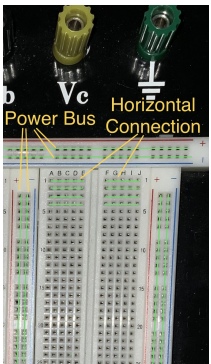
\includegraphics[width=0.3\textwidth]{Aufbau.png}
        \caption{Darstellung des Steckbretts \cite{ap51}.}
        \label{fig:Aufbau}
    \end{center} 
    \end{wrapfigure}
Die verschiedenen Schaltkreise werden auf einem Steckbrett aufgebaut. 
Die vertikalen Verbindungen werden für die Stromversorgung und die Erdung verwendet. Die horizontalen Verbindungen 
sind in der gleichen Reihe miteinander verbunden. Dies ist durch grüne Linien in \autoref{fig:Aufbau} dargestellt.
Darüber hinaus können verschiedene Reihen mit Überbrückungsdrähten verbunden werden. 
Der gesamte Versuchsaufbau besteht abgesehen von dem Steckbrett zusätzlich noch aus einem Funktionsgenerator, der für eine Gleichspannung sorgt, 
einem Multimeter und einem Oszilloskop. Die Operationsverstärker können auf das Steckbrett gesetzt werden.
\\
Der genaue Aufbau variiert während des Experiments, sodass dieser im Rahmen der Durchführung genauer erläutert wird.